\section{Методы измерения}
\label{mes_mthods}
\subsection{SVD}

\begin{wrapfigure}{r}{0.5\textwidth}
    \centering
    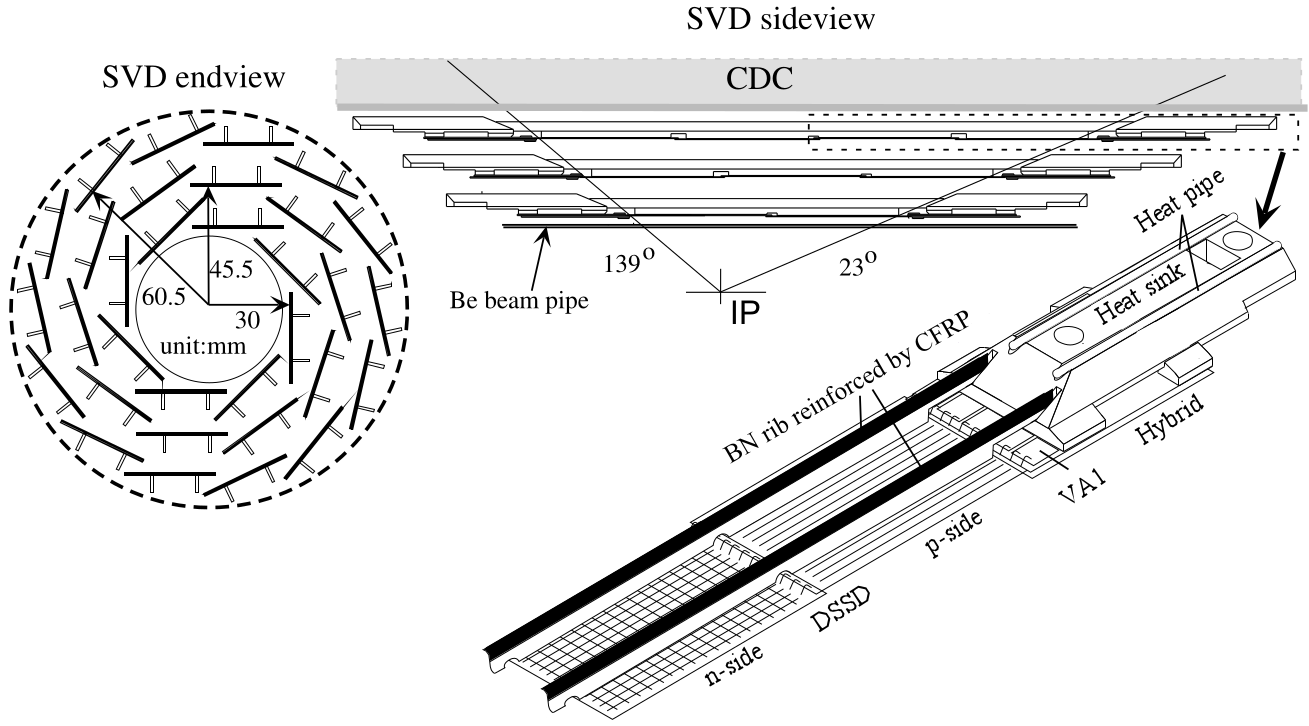
\includegraphics[width=0.48\textwidth]{img/SVD.png}
    \caption{Схематическое изображение SVD.}
    \label{the:SVD}
\end{wrapfigure}

Кремниевый вершинный детектор (рис. \ref{the:SVD}), расположенный непосредственно у точки взаимодействия, 
служит для определения её точного местоположения. Он состоит из тонких слоёв, охватывающих угловой диапазон от $23^\circ$ до $139^\circ$, 
расположенных внахлёст и разделённых на секции, в которых при пролёте частиц 
образуются электронно-дырочные пары. Благодаря большому сечению взаимодействия, 
высокой плотности материала и низкой энергии взаимодействия, полупроводниковые 
детекторы обладают высокой точностью при измерении широкого диапазона энергий частиц.
Это позволяет определять точку взаимодействия с точностью до $100\mu m$. 
Однако, несмотря на значительно более высокую точность по сравнению с газовыми детекторами, 
монтаж большого количества слоёв усложнён из-за возможных сильных отклонений 
трека в результате многократного взаимодействия с плотными кристаллами кремния.

\subsection{Система идентификации заряженных адронов}

Система включает в себя три основные детектора: CDC, TOF и ACC.

\begin{wrapfigure}{r}{0.5\textwidth}
    \centering
    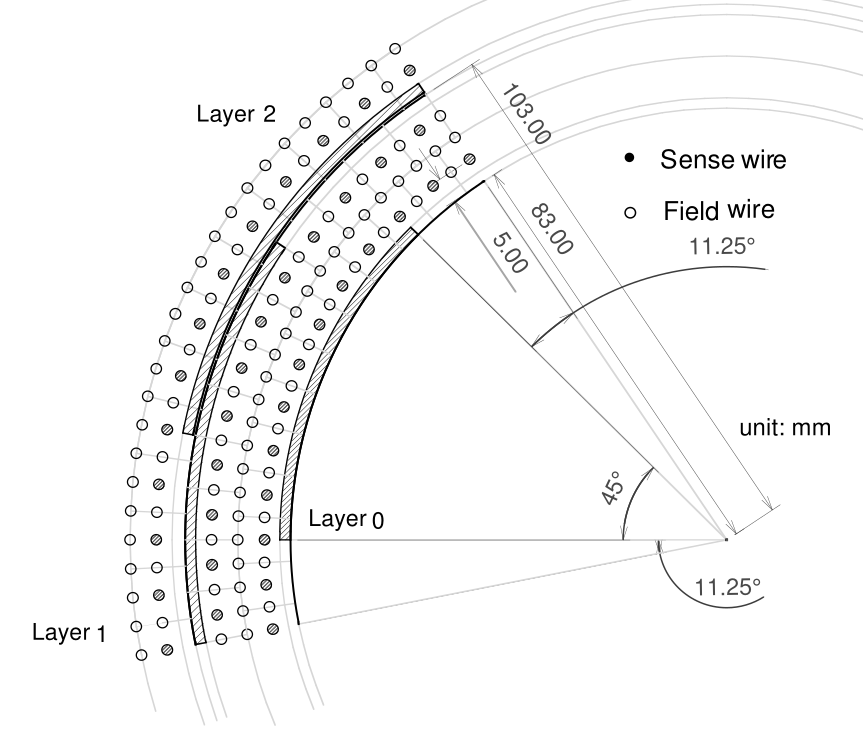
\includegraphics[width=0.3\textwidth]{img/CDC.png}
    \caption{Конфигурация слоёв проволок в центральной дрейфовой камере (CDC).}
    \label{the:CDC}
\end{wrapfigure}

CDC (центральная дрейфовая камера) представляет собой вытянутый цилиндр, слегка деформированный для 
эффективного охвата полярного угла от $17^\circ$ до $150^\circ$. Камера заполнена смесью газов $He$ и $C_2H_6$, 
что минимизирует влияние на трек частицы и обеспечивает максимальную эффективность ионизации. 
Высвобождающиеся электроны движутся к тонким алюминиевым проволокам, натянутым внутри объёма CDC (рис. \ref{the:CDC}). 
На проволоки подаётся напряжение порядка $20kV/cm$. При достижении электронами проволок происходит лавинное умножение электронов, 
что фиксируется системой. Вся камера находится в магнитном поле с индукцией около $1.5 T$, что позволяет измерять импульс 
частицы по кривизне её трека. Также потери энергии на ионизацию позволяют оценить массу частицы, что, в свою очередь, 
помогает в идентификации заряженных частиц.

\begin{wrapfigure}{l}{0.5\textwidth}
    \centering
    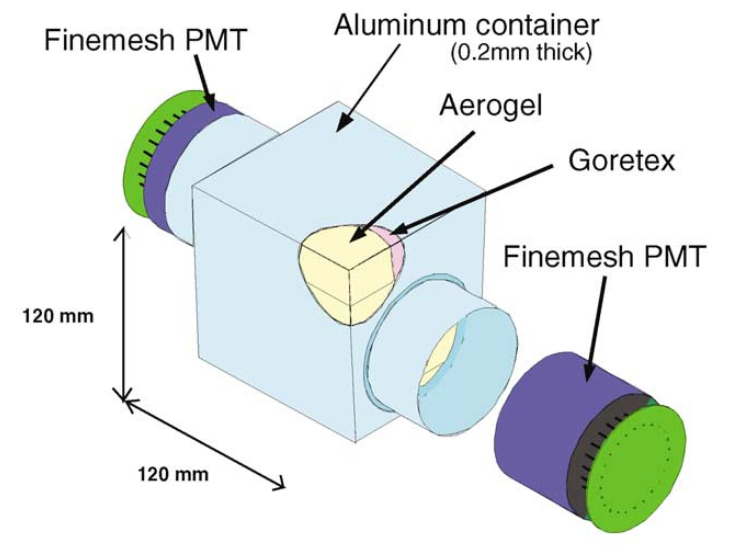
\includegraphics[width=0.4\textwidth]{img/ACC.png}
    \caption{Детектор черенковского излучения (ACC).}
    \label{the:ACC}
\end{wrapfigure}

ACC (детектор черенковского излучения) состоит из отдельных модулей размером $12\times12\times12$ см, 
расположенных цилиндрически и разделённых на 240, 240 и 360 модулей, ориентированных под различными углами для эффективного 
захвата частиц. Дополнительно имеется 228 счётчиков, установленных на торцевой стороне для учёта частиц, движущихся в 
определённом направлении из-за особенностей распределения импульса. Частицы, пролетающие через арогелевые среды, заполняющие 
модули ACC, возбуждают фотоны, длина волны которых зависит от заряда, импульса и массы частицы.

TOF (времяпролётный детектор) --- это система пластиковых сцинтилляционных счётчиков, 
расположенных вдоль всей системы, предназначенная для разделения каонов и пионов при импульсах менее $1.2 GeV$. 
Такое разделение основано на принципе работы: отклик в 128 сцинтилляционных счётчиках сравнивается с 
длиной трека, рассчитанной путём экстраполяции из трековой системы.


\begin{figure}[!htb]
    \centering
    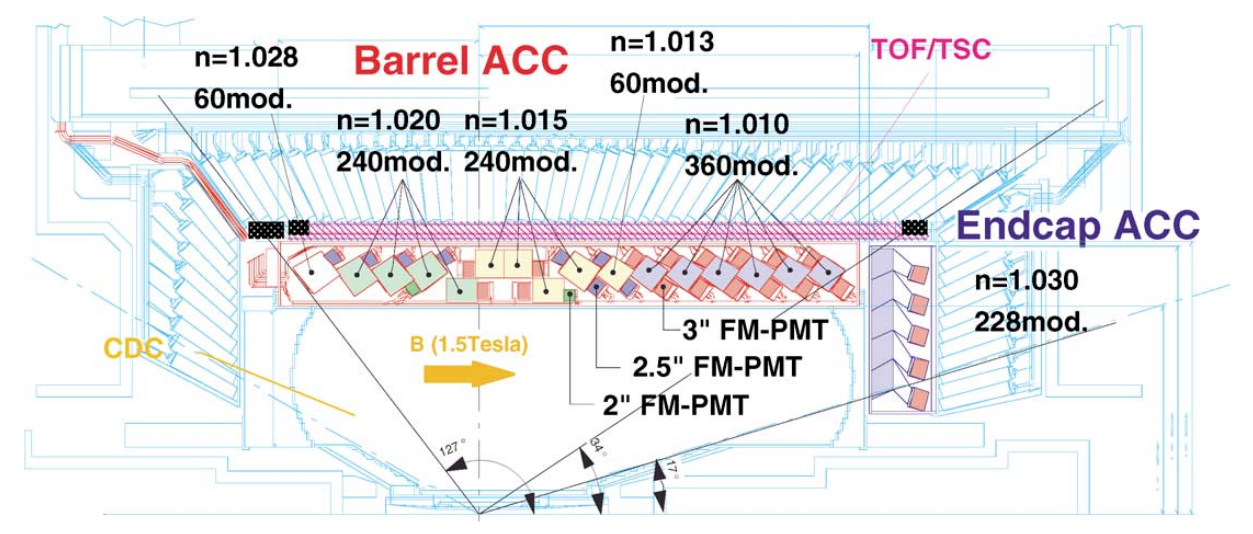
\includegraphics[width=1\linewidth]{img/Ch_hadr_id.png}
    \caption{Полная система идентификации заряженных частиц (ACC, CDC и TOF).}
    \label{the:ch_hadr_id}
\end{figure}

\begin{wrapfigure}{r}{0.5\textwidth}
    \centering
    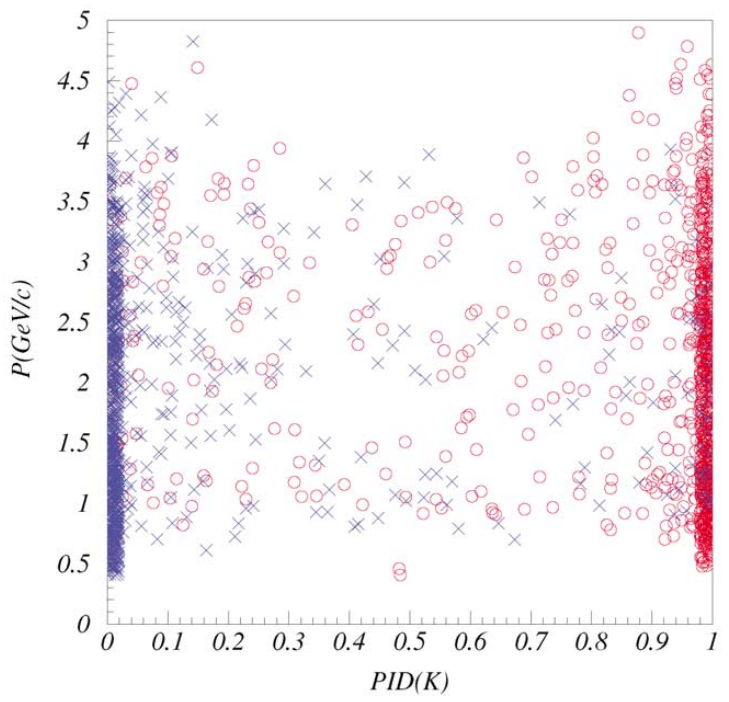
\includegraphics[width=0.7\linewidth]{img/L_P.png}
    \caption{Рапределение $PID$ для $K$ - синие кресты и $\pi$ - красные окружности}
    \label{the:li}
\end{wrapfigure}

Следующий абзац применим для всех подсистем Belle не только для ACC, CDC и TOF, 
но входе идетефикации заряженных адронов эти при играют наибольшую роль и пример разобран них.
На основе данных ACC, CDC и TOF, вычисляются значения правдоподобия трека, классификации его как конкретной частици, 
для каждого детектора: $L_{ACC}(p,a)$ для ACC, 
$L_{TOF}(p,a)$ для TOF и $L_{CDC}(p,a)$ для CDC, где $p$ --- это гипотеза о типе частицы, $a$ --- трек.
(аналогичные значения правдоподобия формируют все под системы Belle). 
Общая функция правдоподобия рассчитывается как произведение отдельных функций 
$L(p,a) = L_{ACC}(p,a) \cdot L_{TOF}(p,a) \cdot L_{CDC}(p,a)$.
Затем для двух гипотез о типе частицы вычисляется показатель $PID$ (отношение правдоподобий):
\begin{equation}
    \mathfrak{L}(a)_{p_1/p_2} = \frac{L(p_1,a)}{L(p_1,a) + L(p_2,a)},
\end{equation}
где $p_1$ и $p_2$ — два возможных типа частицы, $a$ --- трек.

\subsection{ECL (CsI)}

Электромагнитный калориметр ссотои из сегментов направленных в к точке взаимодействия. 
Система создана для идентефикации и измерения энергий фотононов и электронов 
рождаемых в большом количестве входе электроно позитронноый анигиляции. 
Принцип работы основан на рождении электромагнитного ливня в ходе ракции
$e^- \to \gamma e^- \to 2e^- e^+ \to ...$. В силу своего раположения и устройства 
исправно идентефицируются частици с импульсом более $0.6 GeV$, так как до этого частицу необходимо 
преодотеть SVD, CDC, TOF, ACC и слои металла отделяющих их.

\subsection{KLM}

Наиболее далеко от точки взаимодействия установлен KLM. Его главной задачей
является идентификация мюонов, которые пролетают калориметр без развития 
ливня, что уменьшает различия от заряженных адронов и затрудняет идентификацию.
Дектектор состоит из 14 железных слоев, $K_L$ мезоны проходя через слои металла
порождают ливни инов. При этом частици идентефицируются по глубине прникнования 
в слои металла. Аналогично как для ECL эффективно идетефицировать KLM способен 
частици с импульсами более $1 Gev$.





